\documentclass[11pt]{article} % use larger type; default would be 10pt
\usepackage[utf8]{inputenc} % set input encoding (not needed with XeLaTeX)

%%% PAGE DIMENSIONS
\usepackage{geometry} % to change the page dimensions
\geometry{a4paper} % or letterpaper (US) or a5paper or....
\newcommand{\tab}{\hspace*{2em}}

%%% PACKAGES
\usepackage{graphicx} % support the \includegraphics command and options
\usepackage{wrapfig} % Figure wrapping
% \usepackage[parfill]{parskip} % Activate to begin paragraphs with an empty line rather than an indent
\usepackage{booktabs} % for much better looking tables
\usepackage{array} % for better arrays (eg matrices) in maths
\usepackage{paralist} % very flexible & customisable lists (eg. enumerate/itemize, etc.)
\usepackage{verbatim} % adds environment for commenting out blocks of text & for better verbatim
\usepackage{subfig} % make it possible to include more than one captioned figure/table in a single float
\usepackage{url}
\usepackage{enumerate}
\usepackage{cleveref}  %cites figures intelligently
\usepackage{import} % document structuring
\usepackage{float}  %These two ensure that table position follows text by specifying {table}[H]
\restylefloat{table}

%CODE LISTINGS
\usepackage{color}
\usepackage{listings}

\lstset{
	tabsize=4,
%	language=matlab,
        	basicstyle=\scriptsize,
%     	upquote=true,
       	aboveskip={\baselineskip},
        	columns=fixed,
        	showstringspaces=false,
        	extendedchars=true,
        	breaklines=true,
	prebreak = \raisebox{0ex}[0ex][0ex]{\ensuremath{\hookleftarrow}},
	frame=single,
        	showtabs=false,
        	showspaces=false,
        	showstringspaces=false,
        	identifierstyle=\ttfamily,
        	keywordstyle=\color[rgb]{0,0,1},
        	commentstyle=\color[rgb]{0.133,0.545,0.133},
        	stringstyle=\color[rgb]{0.627,0.126,0.941},
	language=C++
}

%%% HEADERS & FOOTERS
\usepackage{fancyhdr} % This should be set AFTER setting up the page geometry
\pagestyle{fancy} % options: empty , plain , fancy
\renewcommand{\headrulewidth}{0pt} % customise the layout...
\lhead{}\chead{}\rhead{}
\lfoot{}\cfoot{\thepage}\rfoot{}

%%% SECTION TITLE APPEARANCE
\usepackage{sectsty}
\allsectionsfont{\sffamily\mdseries\upshape} % (See the fntguide.pdf for font help)
\usepackage{titlesec}
%\titleformat{\subsection}[runin]{\mdseries\bf}{\thesubsection}{1em}{}
%\titleformat{\subsubsection}[runin]{\mdseries\bf\underline\large}{\thesubsection}{1 em}{\vspace{-5 pt}}

\usepackage{footbib}

% (This matches ConTeXt defaults)

%%% ToC (table of contents) APPEARANCE
%\usepackage[nottoc,notlof,notlot]{tocbibind} % Put the bibliography in the ToC
\usepackage[titles,subfigure]{tocloft} % Alter the style of the Table of Contents
\renewcommand{\cftsecfont}{\rmfamily\mdseries\upshape}
\renewcommand{\cftsecpagefont}{\rmfamily\mdseries\upshape} % No bold!

\begin{document}

\part{TimeLapse}
Time-lapse photography is the process by which a camera is set up to watch a particular object for extended periods of time. Instead of the camera taking frames continuously for that period, intervals are specified which are much lower than the normal framerate (e.g. 1 frame per hour). Once the frames are accumulated and played at a normal frame rate (e.g 30 frame per second) then time appears to run fast and lapsing occurs.
The technique has been used to capture crowds of people, traffic, and other everyday entities which at a normal speed seem unimpressionable, but at high speeds become a fast flurry of activity.

There were three approaches I could take to make a TimeLapse application:\\
\tab1. Run the app continuously for the full duration of the time lapse period specified.\\
\tab2. Run the app continuously in the background for the full duration of the time lapse period.\\
\tab3. Schedule the app to run and exit at specified times until the full duration of the time lapse period\\

The first approach would have meant that the application would have been in the main foreground while all the frames were being taken. If I wanted to capture a frame every hour for two days, then the app would have to be open and active for that entire time. This would be a waste of RAM, since the application will occupy a chunk of memory for two days without actually doing any work for most of that time. This will also occupy window space since the application UI will be active in this time, which is a major problem because the user may unwittingly close the application preventing it from completing it's job.

The second approach is the same as the first; waste of RAM over an extended period of time, but this time the window of the application is hidden and so the user will not be able to accidentally cancel the task once it is set. Doing this is very easy, since in Qt all one has to do is get rid of the myClass->show() function to run the app in the background. But as before, this is not optimal and wastes RAM.

This leaves the third option, which is to set scheduled events for the app so that it starts and stops at specific times with minimal usage of system resources. The question now is how to enable the MotionDetector to do this.

\section{Command Line Switches}
\subsection{Argument parser}

Qt (like most SDk's) places all the arguments to a program in a list of some kind. In Qt, the arguments are accessed via QApplication::arguments() which returns the arguments in a QStringList (very similar to an ArrayList in Java).

My first step was to create a CommandLine class. This class would take a reference to the QStringList and check the tokens within that for certain key flag values. The key flag values needed would have to be same options that can be specified by the user, and so I settled with the standard convention of providing longhand and shorthand names for flags with '- -name' and '-n' respectively:
\begin{frame}[fragile]
\lstinputlisting[title=\textbf{Source Code: help.sh}]{../Code/commandline/help.sh}
\label{frame:help}
\end{frame}

To search for flags, I used QStringLists' ".contains(key)" method which performs a search over all the tokens in the argument list. This can be very slow, especially if other less important flags are searched first. 
For this reason, flags such as '--help' or '--version' were the first two flags to be searched, since these will print a quick message and then terminate without having to check for further flags.

The other flags followed a different logic:
\begin{frame}[fragile]
\lstinputlisting[title=\textbf{Source Code: checkflag.cpp }]{../Code/commandline/checkflag.cpp}
\end{frame}
 First a default value would be set (in this case 5) for the flag\_value, then a search would commence within the if statement.  The '.indexOf(key)' method would find the index of the flag in the array, or else return -1 if not found. I followed the convention where I would first check for the shorthand name first, and then the longer one since I reasoned that it was less effort to type a shortflag than a longer one, and was thus more likely to occur. This is useful, since C++ supports short-circuit evaluation and so if the first condition is deemed true, it will not need to search the other end of the OR statement.

The flag\_value is then assigned the integer (or other type) version of index after the flag (e.g. We want to grab the 3 from the argument '--flag 3'). In Qt, this is returned as 0 if it could not convert it properly and so some error checking needs to be performed.

\subsubsection{Switch Detection}
Once the flag has had all the useful arguments taken from it, it is then {\it removed} from the argument array in order of highest index for flag, to lowest index for flag (the flag name). This order is necesary because when you remove from an Array at a certain index, all the indexes above it are shifted down meaning you now have to subtract by 1 to access a certain item from the higher indexes which can lead to errors. It is therefore far easier to remove from high index to low index to ensure that the lower indexes are unaffected by changes in the higher indexes.

Why is removal even important here? It's an optimization. By removing the arguments from the array after using them, future searches to that same array for different flag values will be {\it faster} because there are less items to check. This also gives another benefit in that if the user misspells or enters an unknown flag, it will be left over in the argument array , and so the program can notify the user precisely of which flags were not recognised and which one's were:
\begin{frame}[fragile]
\lstinputlisting[title=\textbf{Source Code: unknowns.cpp }]{../Code/commandline/unknowns.cpp}
\end{frame}

So if the user types into a shell:\\
' motiondetect -m 7 --size 320 240 --roger the dodger -w 100'\\
The app will spit out the following error:\\
'Could not parse: --roger the dodger\\Please try --help for more info '

since these will be the leftover arguments that were left in the argument list. Had all the flags been valid, the argument list would have been empty.

\paragraph{Terminal Colours\\}{
To make the commandline look as interesting as possible I also implemented colours into the shell. Fremantle uses the busybox shell by default, which is a lightweight shel that comes prepackaged with many standard utils such as 'ls' 'mv' 'cp' and so forth which are symlinked to /usr/bin/ so as to appear independent of busybox.
Busybox also shares the same as terminal colour codes as Bash, which are called via non-printing escape sequences which are enclosed in \textbackslash[\textbackslash033[ and \textbackslash] pairs.
Using the following colour codes in \cref{tab:colorcodes}, different colours could be printed

\begin{table}[H]
\centering
\begin{tabular}{| r | l |}
\hline
\multicolumn{2}{|c|}{\bf Color codes} \\
\hline
char red[ ] &"\textbackslash033[0;31m\textbackslash033[1m"\\
char cyan[ ] &"\textbackslash033[0;36m"\\
char yellow[ ] &"\textbackslash033[0;33m"\\
char green[ ] &"\textbackslash033[0;32m"\\
char stop[ ] &"\textbackslash033[0m"\\
\hline
\end{tabular}
\caption{Red is a longer sequence than the other colours because default red was not very visible, so I made it {\bf bold} too by appending \textbackslash033[1m" to it.}
\label{tab:colorcodes}
\end{table}

With this framework I could then control what colours I wanted to use by simply calling:\\
cout  yellow \(\langle\langle\) "Warning:" \(\langle\langle\) green \(\langle\langle\) "This shell supports" \(\langle\langle\) cyan \(\langle\langle\) "multiple"\(\langle\langle\)  red \(\langle\langle\) "colors!" \(\langle\langle\) stop \(\langle\langle\) endl;

The stop colour at the end is neccesary to reset the shell to its default color, otherwise the last color set will be maintained for the next message which may not be desirable.

\begin{figure}[H]
	\vspace{-10pt}
	\begin{center}
		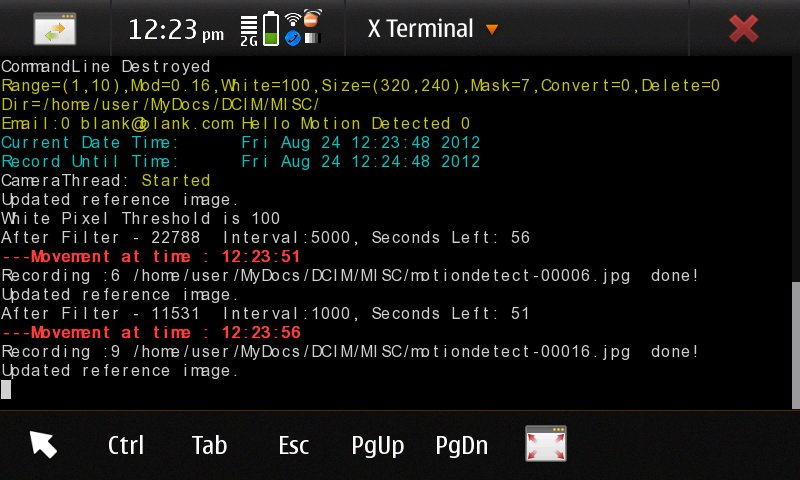
\includegraphics[width=0.8\textwidth]{../images/commandline/commandscreen.jpg}
	\end{center}
	\vspace{-20pt}
	\caption{Screenshot fom phone}
	\label{img:command}
	\vspace{-10pt}
\end{figure}

One of the main benefits of having a commandline implementation is that enables remote usage. A user can simply ssh or telnet into the phone from another machine and start and control the application from the shell on their own computer. The colours will also print correctly too.

}
\subsubsection{Reusing exiting variables}

For standard motiondetection commandline calls such as mask, whitepixel, size, etc as shown in help.sh on page~\pageref{frame:help}, individual variables were created to hold these values, which were mirror variables for the same ones in the CameraThread. When the Commandline finishes parsing arguments it switches flow control back to the motiondetector (main window UI) class which then reassigns these variables to those of the camerathread as shown below:
\begin{frame}[fragile]
\lstinputlisting[title=\textbf{Snippet from MotionDetector (mainwindow UI) }]{../Code/commandline/commandtoops.cpp}
\end{frame}
The main MotionDetector class does not have variables in the header file that hold all the variables, like CommandLine and Operations (the camera thread) do. MotionDetector is simply a UI class, it acts as a waypoint or a go-between for connecting commandline arguments to the camerathread.

When commandline arguments are not given, the 'commands' pointer is initialised to zero and is thus empty. In this case the UI is active and so Operations gets its values directly from the UI. When the pointer is not empty, the UI is ignored and Operations gets its values directly from CommandLine. An exit slot is also connected in this case, so that when the camera thread finishes, the entire application safely closes (which overrides the default finish behaviour, where the UI simply becomes active and listens for input again).

The real trick is when we want to perform a timelapse operation. Timelapse operations need only five arguments:
\\ Image size, frame rate, convert images to movie,  delete images after conversion, and end date.
Image size, convert and delete are variables used in motiondetection operations, so these values can be assigned correctly. But what do we do with frame rate and end date? These variables do not exist for motion detection operations, and it would be wasteful to create new variables for them, because as discussed above; whatever variables we create in commandline we must also create in Operations (the camera thread). Creating a framerate and enddate variable will be making variables that will be unused most of the time.

Instead, we reuse the one's that exist already but are not being used. To pass framerate into operations, we simply pass it as a mask variable (they are both integers) and to pass the end date we pass it as a time variable that is normally used in the motiondetector as duration. This reduces the number of class variables and in turn reduces overhead. Should I wish to create further options for the timelapse part of the app I can just slot them into the currently inactive motiondetector variables.

The camera thread needs to know whether it will do





\paragraph{Why echoing the same command at differeint intervals?}
\section{Scheduled Events}
\subsection{Cron}
\subsection{Cookies, Triggers, Flags}
\subsection{Logic of repeated calls}
\section{Software Battles}
\subsection{Cron Vs Alarmd}
\subsection{qDebug vs std::cout}
\subsubsection{Message Handlers}
\section{Optimisations/Error Proofing}
Commandline not called until arguments!=0, then it is destroyed intelligently.

\end{document}